\documentclass[main.tex]{subfile}

\begin{document}
\section{Results} 
\label{sec:results}

By visual inspection the following results are observed in the correlation
between each PID constant:

\begin{table}[H]
	\begin{tabularx}{width=\textwidth}{lll}
		\toprule
		$K_p$ & $K_i$ & $K_d$
		\\bottomrule
	\end{tabularx}
	\caption{}
	\label{tab:}
\end{table}

% include the tables of data and images (generated by makeTexFloats.sh)

\begin{table}[H]
\begin{tabular}{ccc}
\toprule
\\ 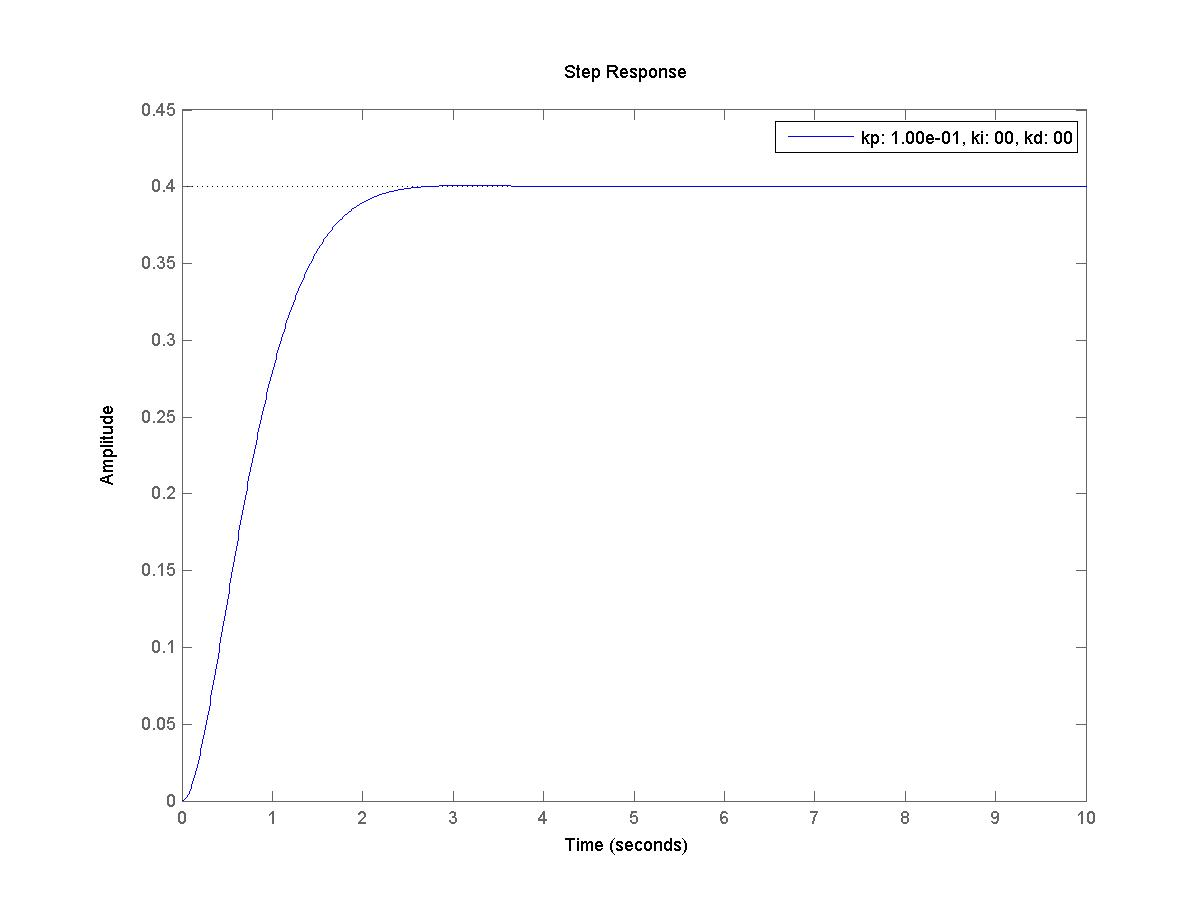
\includegraphics[width=1.8in]{part1-1.jpg} 
& 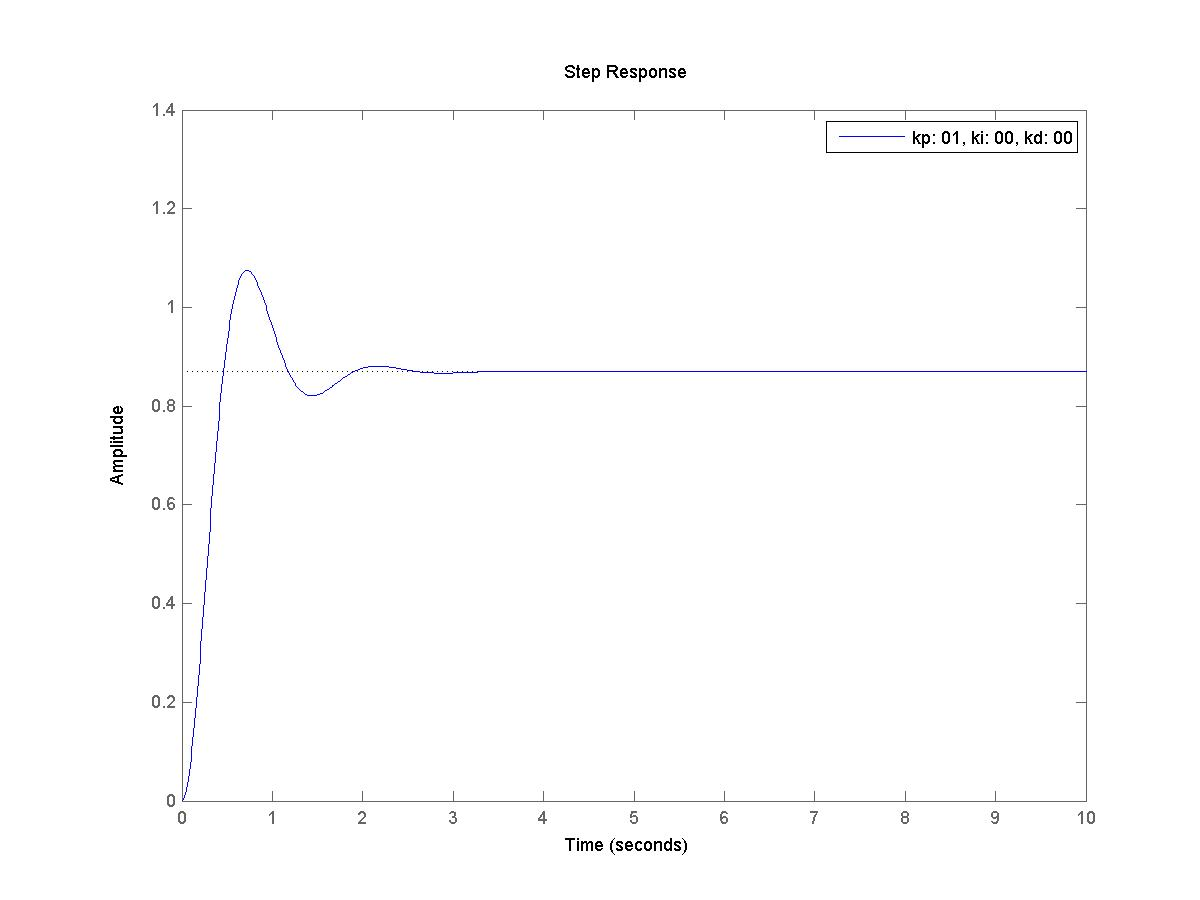
\includegraphics[width=1.8in]{part1-2.jpg} 
& 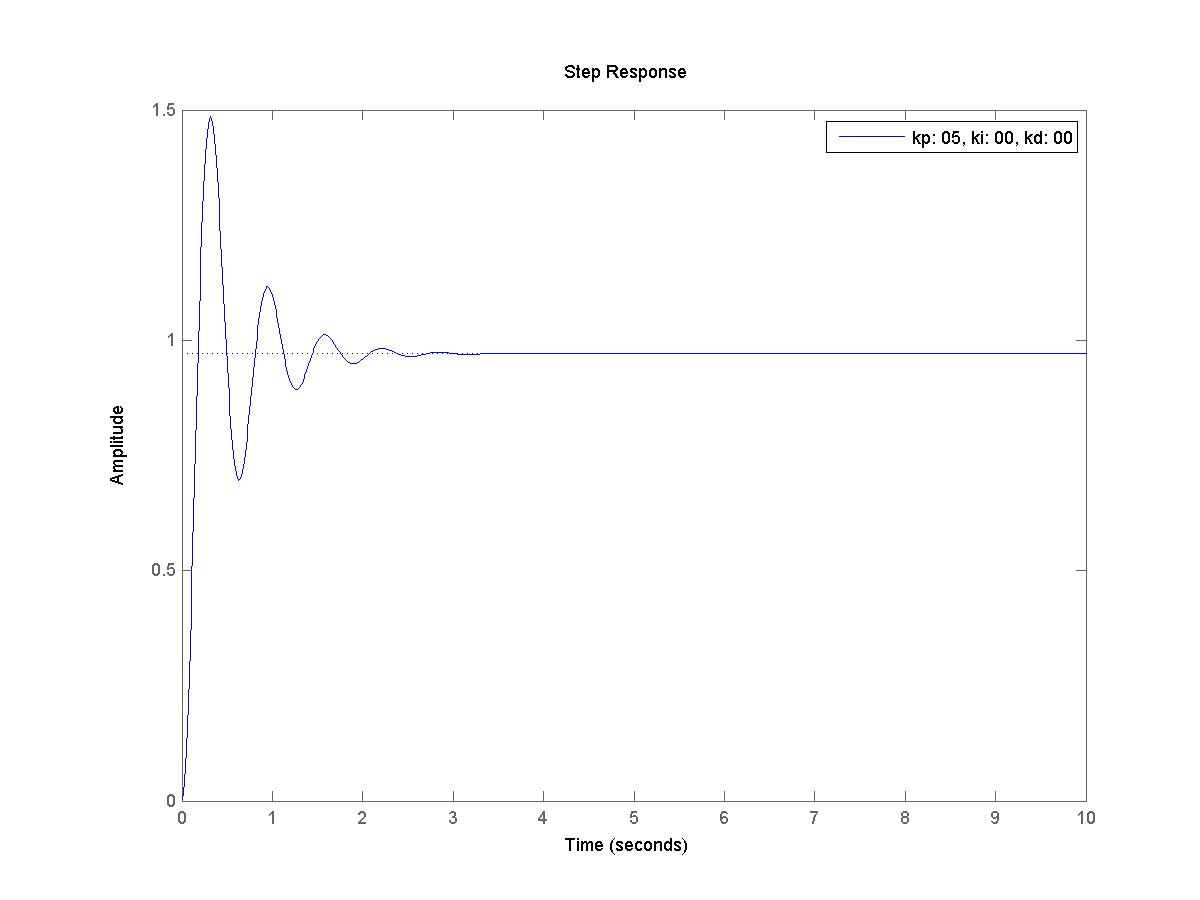
\includegraphics[width=1.8in]{part1-3.jpg} 
\\ 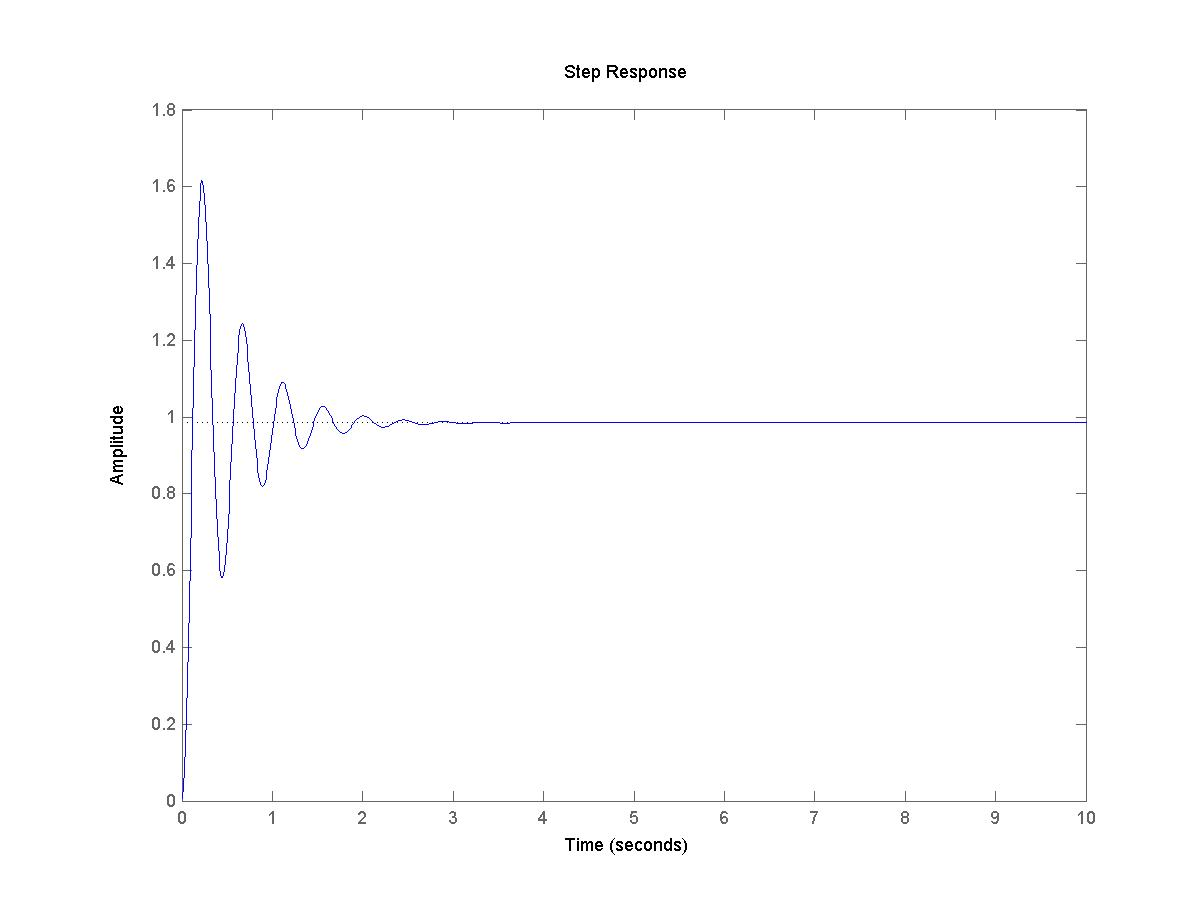
\includegraphics[width=1.8in]{part1-4.jpg} 
& 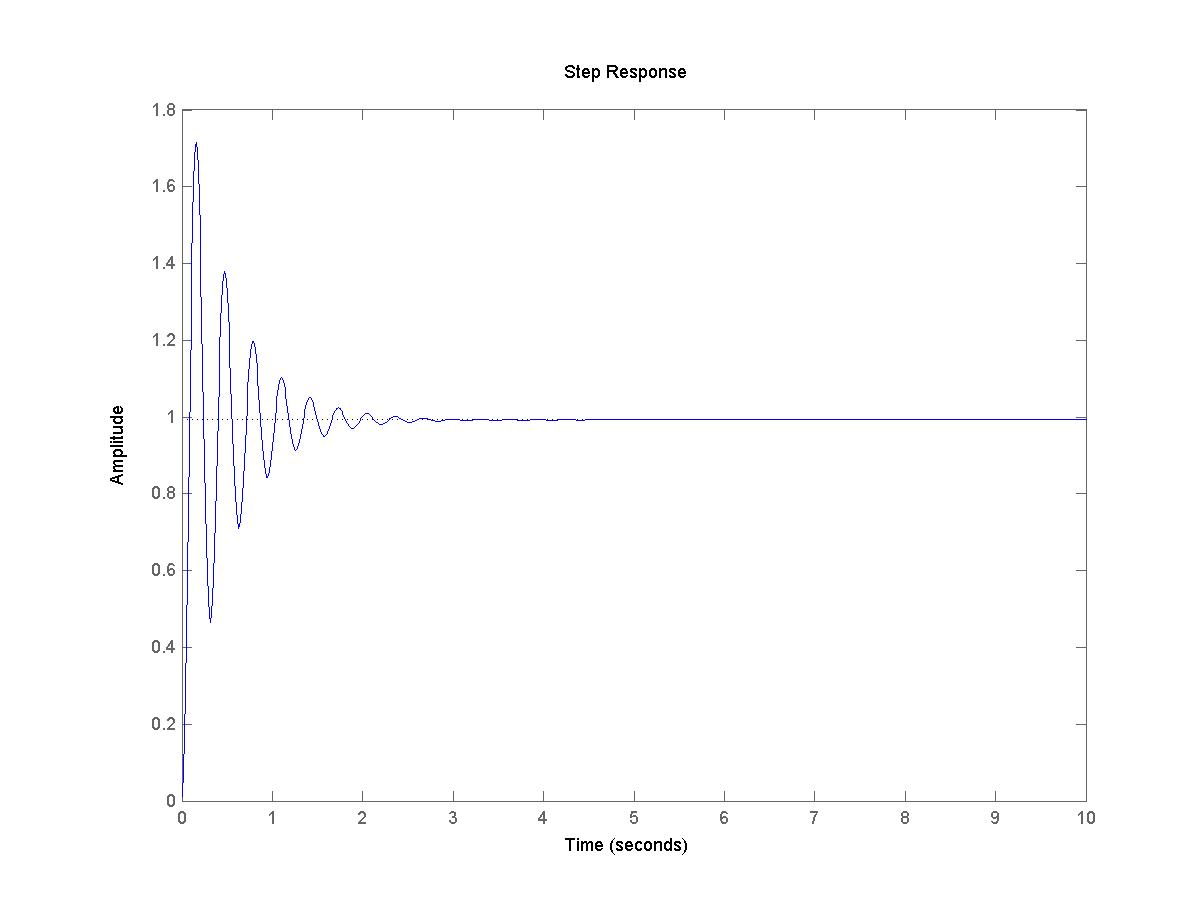
\includegraphics[width=1.8in]{part1-5.jpg} 
& 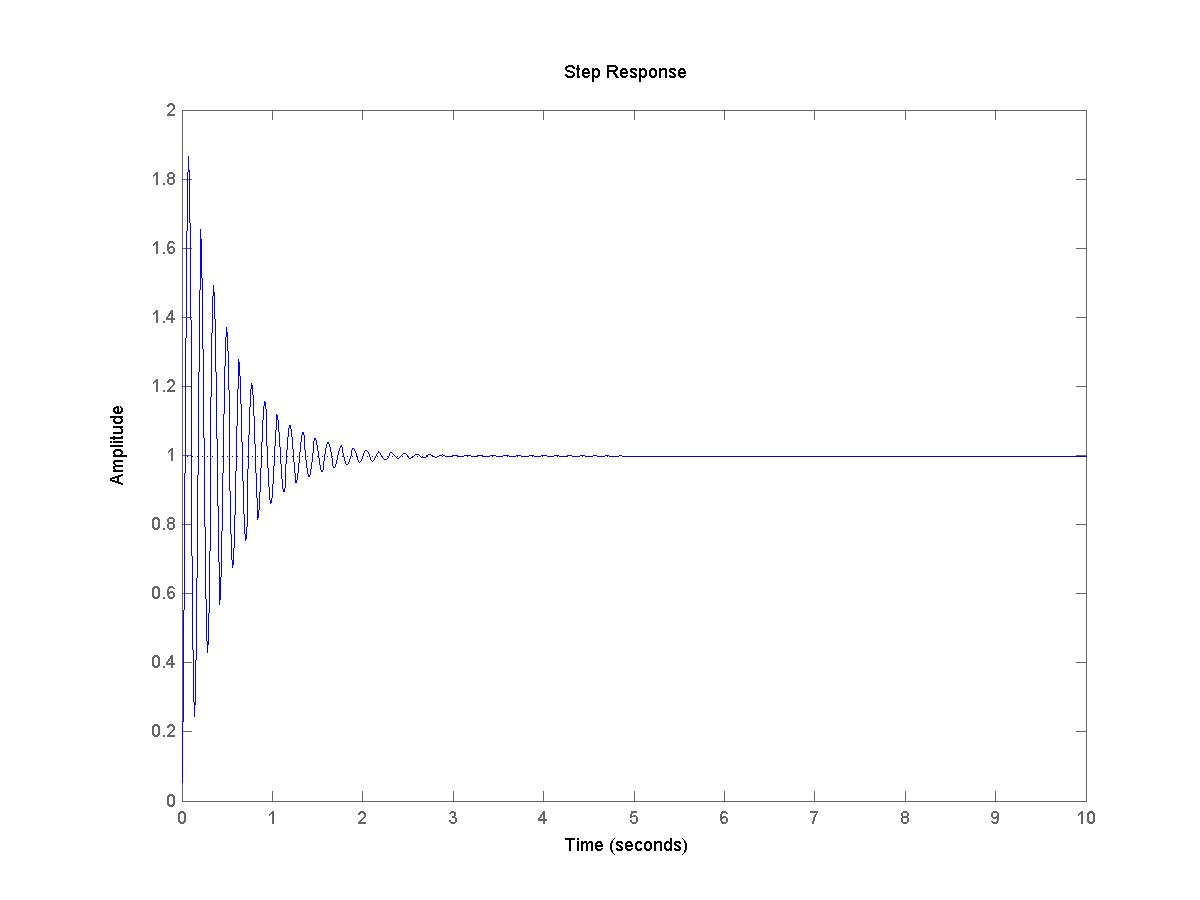
\includegraphics[width=1.8in]{part1-6.jpg} 
\\ 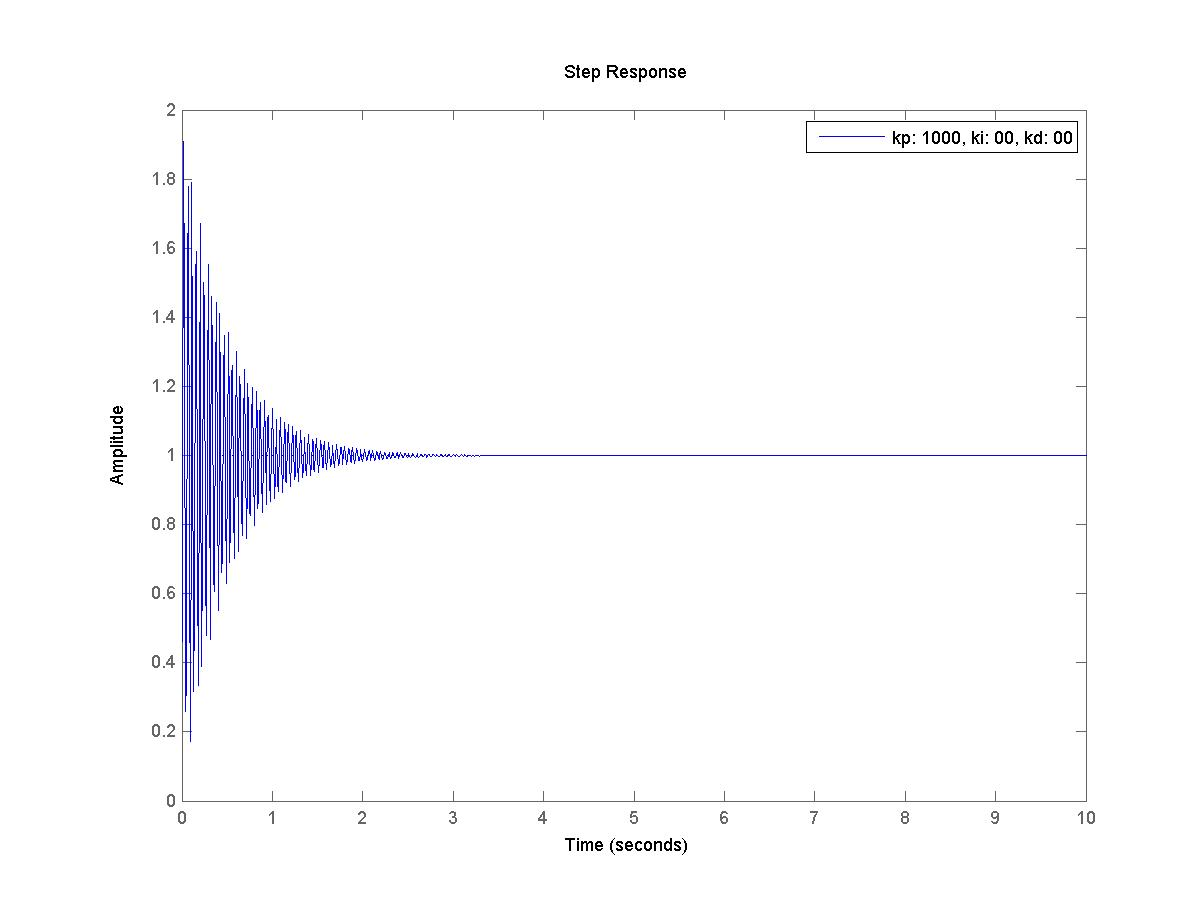
\includegraphics[width=1.8in]{part1-7.jpg} 
\\ \bottomrule
\end{tabular}
\caption{Part 1 Step Responses}
  \label{tab:part1Response}
\end{table}
\begin{table}[H]
	\begin{tabularx}{\textwidth}{XXXXXXXXXX}
		\toprule
		\\ $K_p$ & $K_i$ & $K_d$ & $T_r$ & $T_p$ & $T_s$ & $\%OS$ & $e_{ss}$ 
		& Stable System? & Damping Classification
		\\ \midrule
		
\\\midrule\\0.1&0&0&1.278&3.14&2.074&0.186&0.714&yes&under 
\\\midrule\\1&0&0&0.310&0.72&1.751&23.658&0.534&yes&under 
\\\midrule\\5&0&0&0.118&0.32&1.943&53.130&0.507&yes&under 
\\\midrule\\10&0&0&0.080&0.22&1.839&64.009&0.503&yes&under 
\\\midrule\\20&0&0&0.055&0.16&1.912&72.902&0.501&yes&under 
\\\midrule\\100&0&0&0.023&0.07&1.906&86.883&0.500&yes&under 
\\\midrule\\1000&0&0&0.009&0.02&1.911&90.985&0.500&yes&under 
		\\ \bottomrule
	\end{tabularx}
	\caption{Part 1 PID Results}
	\label{tab:pid1SimResults}
\end{table}
\begin{table}[H]
\begin{tabular}{ccc}
\toprule
\\ 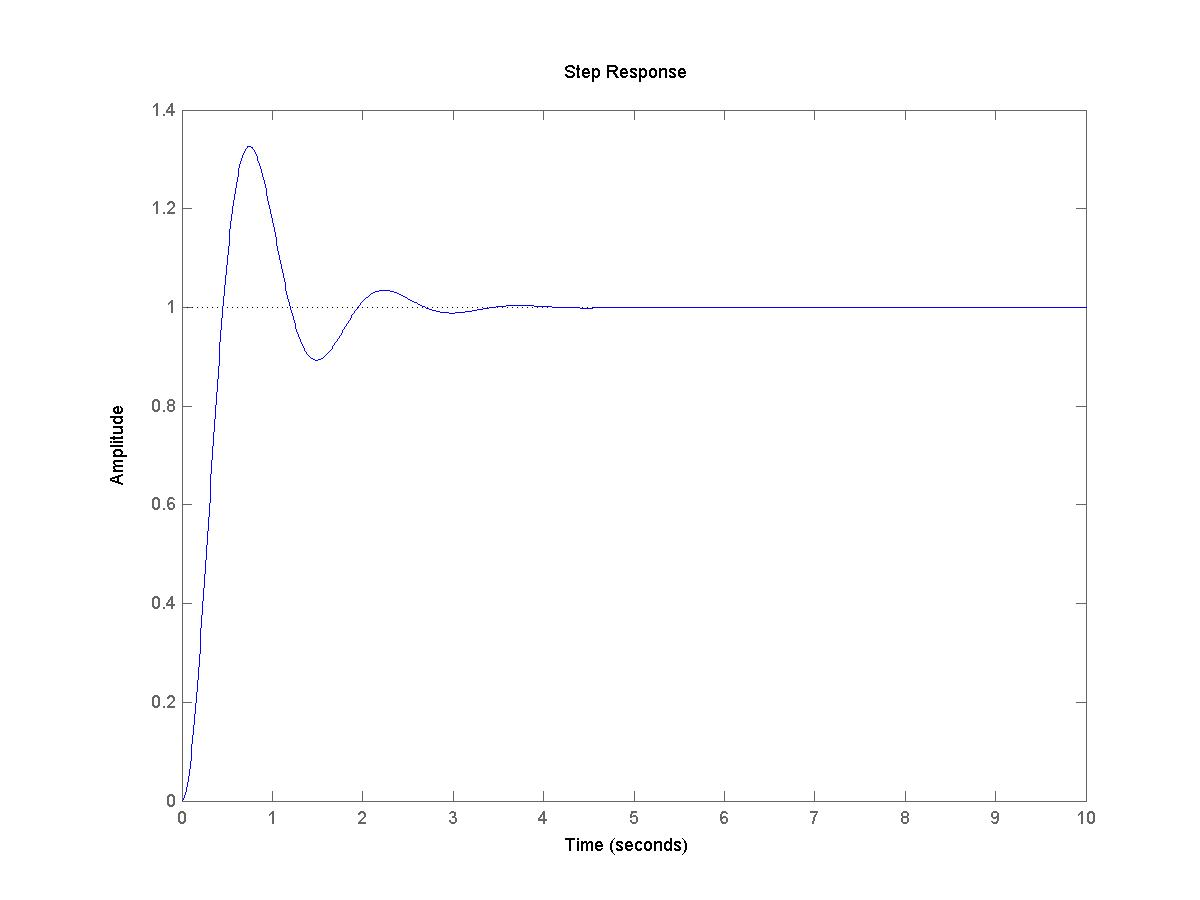
\includegraphics[width=1.8in]{part2-1.jpg} 
& 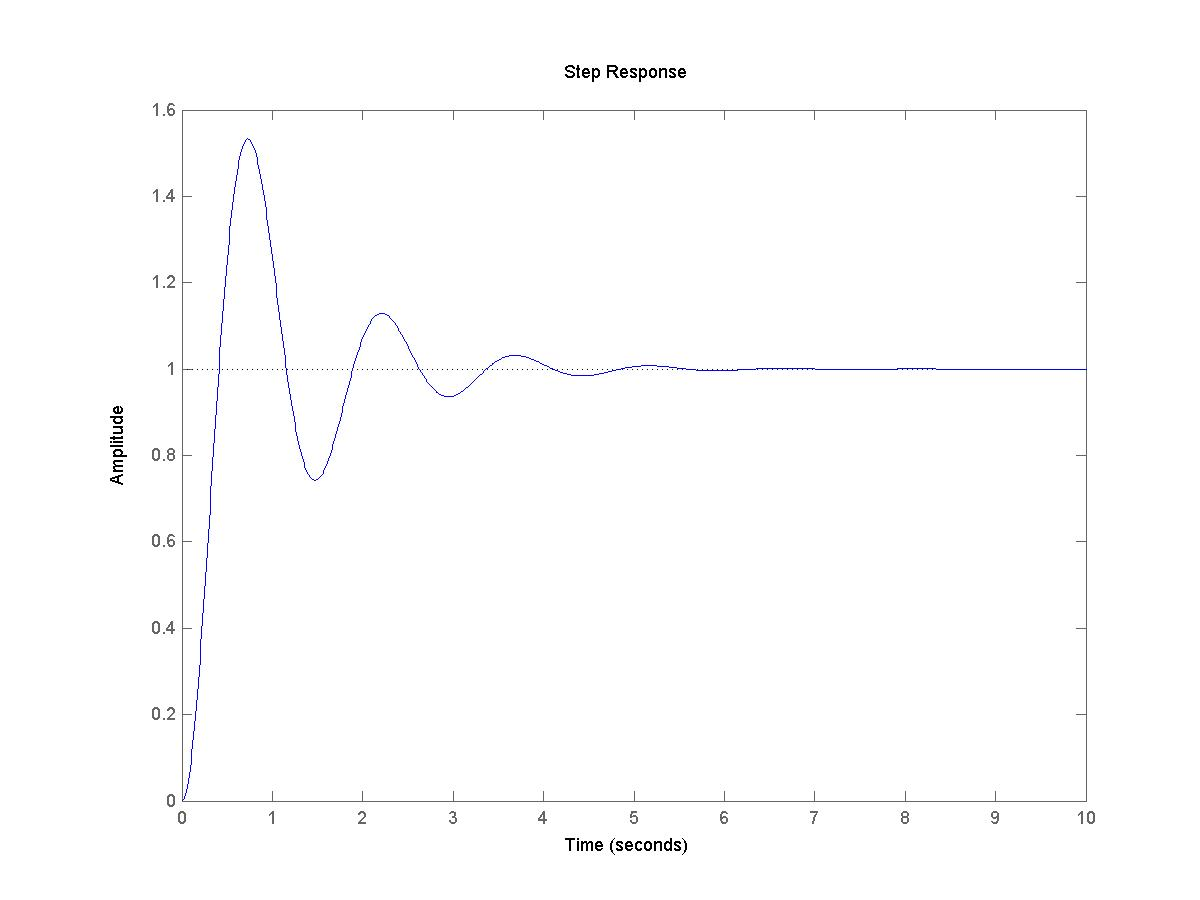
\includegraphics[width=1.8in]{part2-2.jpg} 
& 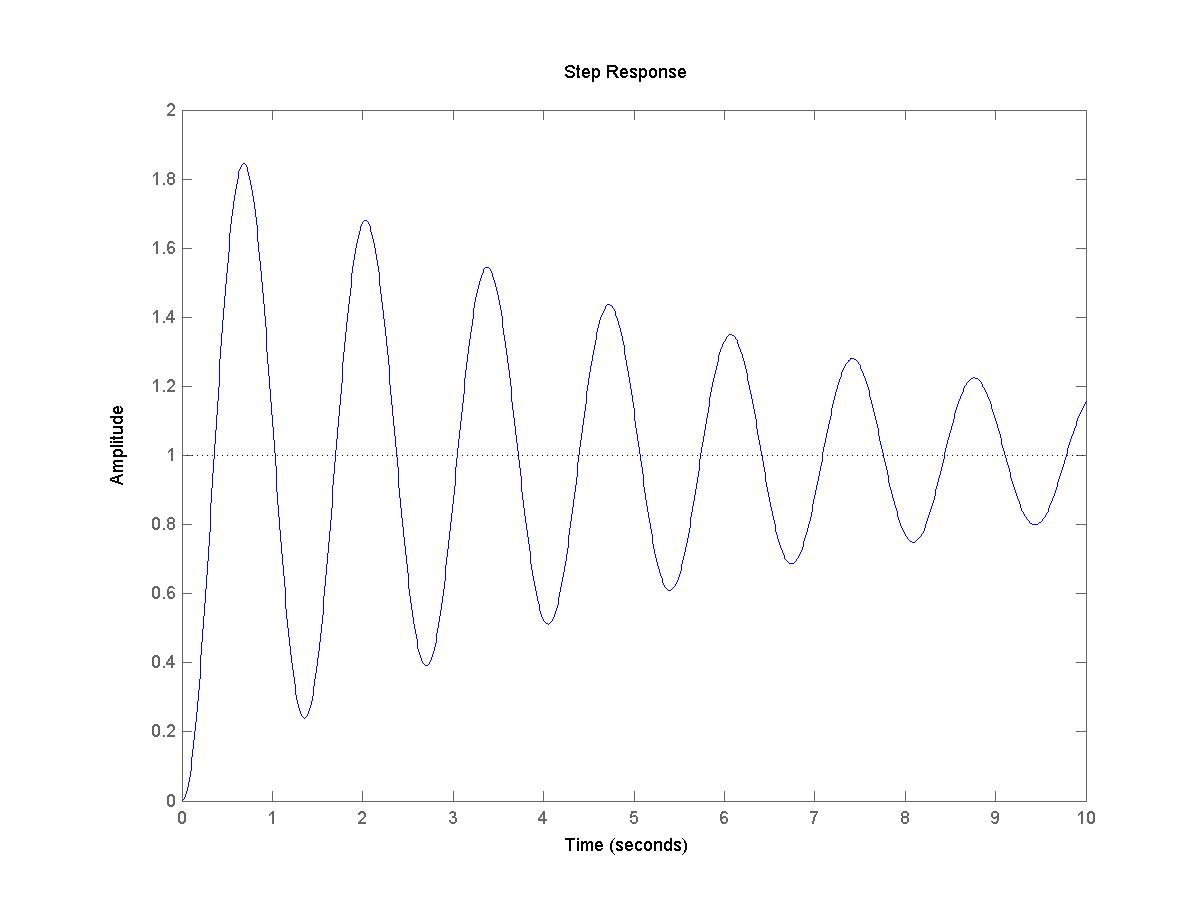
\includegraphics[width=1.8in]{part2-3.jpg} 
\\ 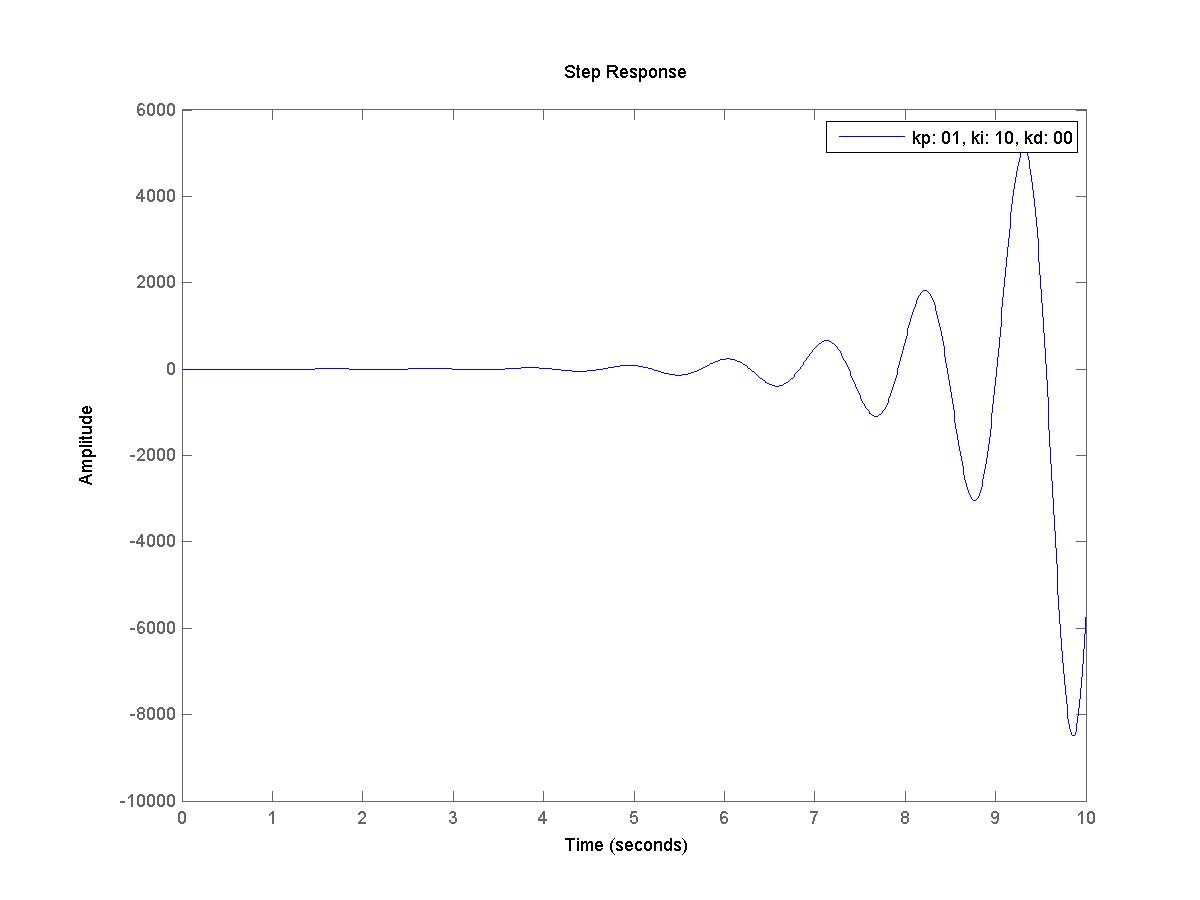
\includegraphics[width=1.8in]{part2-4.jpg} 
& 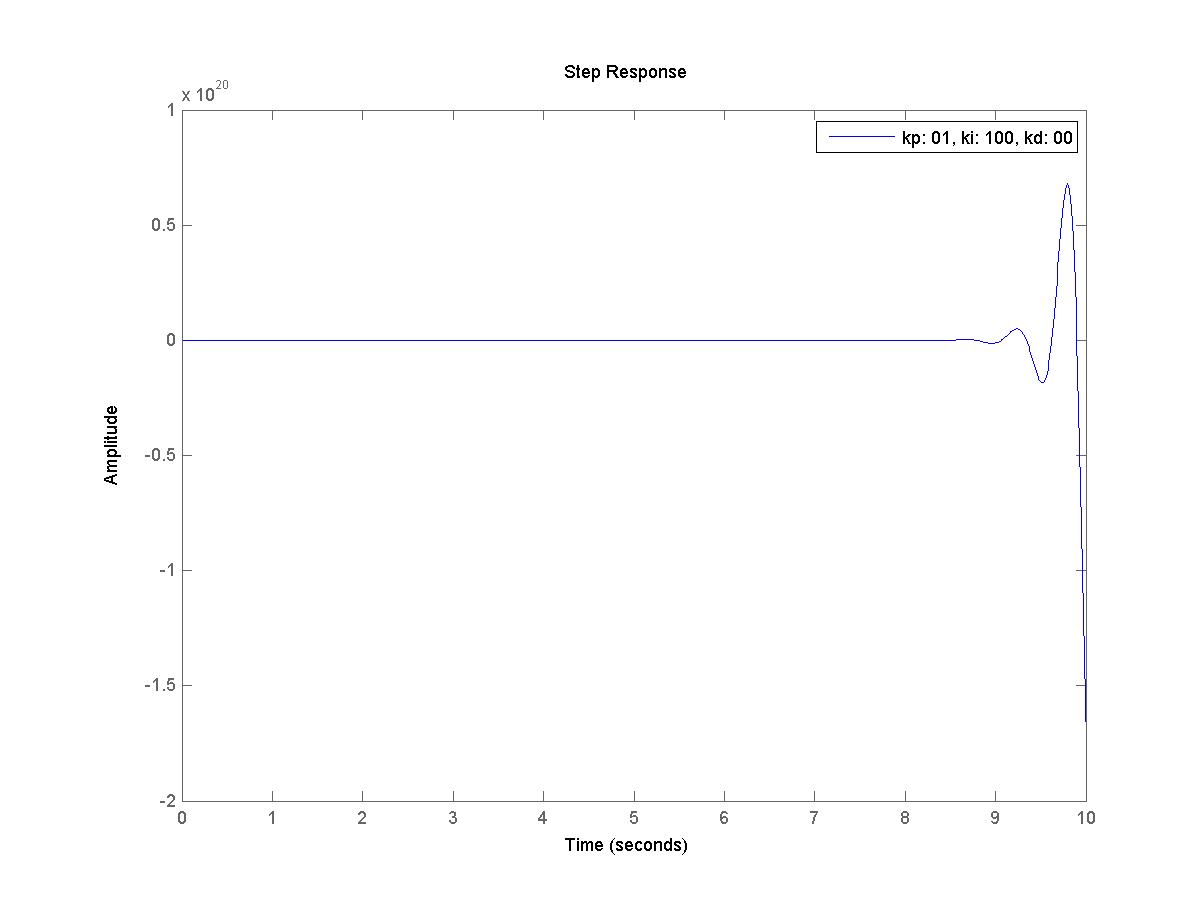
\includegraphics[width=1.8in]{part2-5.jpg} 
& 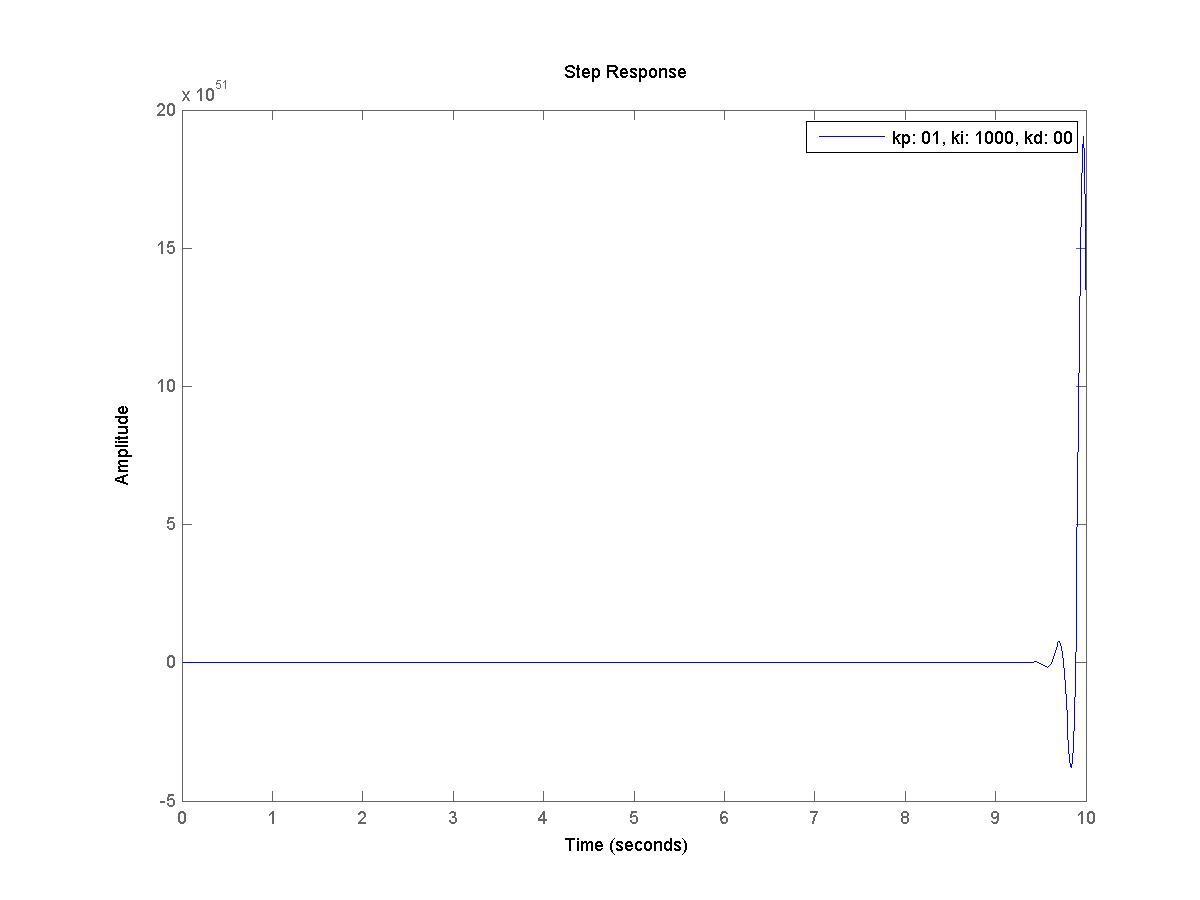
\includegraphics[width=1.8in]{part2-6.jpg} 
\\ 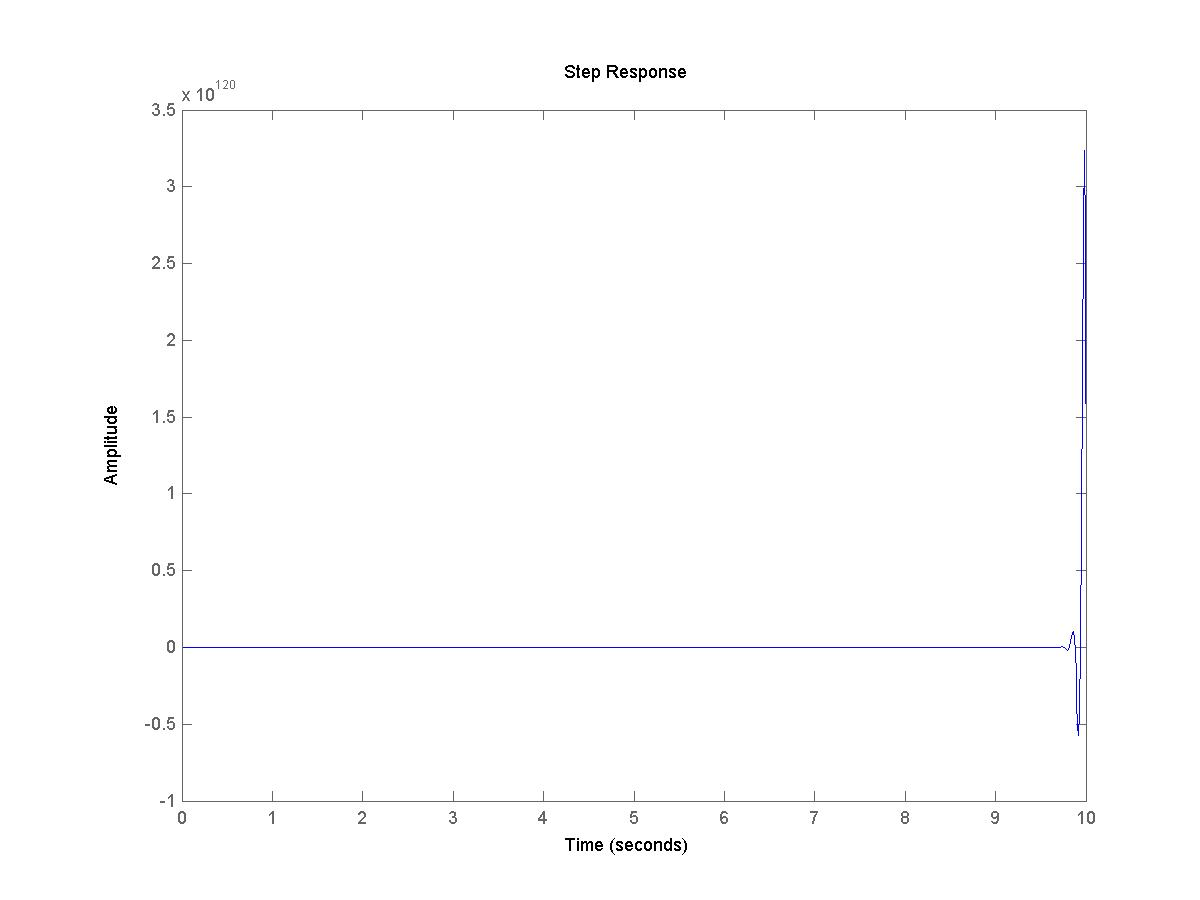
\includegraphics[width=1.8in]{part2-7.jpg} 
\\ \bottomrule
\end{tabular}
\caption{Part 2 Step Responses}
  \label{tab:part2Response}
\end{table}
\begin{table}[H]
	\begin{tabularx}{\textwidth}{XXXXXXXXXX}
		\toprule
		\\ $K_p$ & $K_i$ & $K_d$ & $T_r$ & $T_p$ & $T_s$ & $\%OS$ & $e_{ss}$ 
		& Stable System? & Damping Classification
		\\ \midrule
		
\\\midrule\\1&1&0&0.306&0.75&2.479&32.670&0.5&yes&critically 
\\\midrule\\1&2&0&0.272&0.73&3.904&53.300&0.5&yes&critically 
\\\midrule\\1&4&0&0.257&0.68&9.953&59.493&0.5&yes&critically 
\\\midrule\\1&10&0&2.201&9.86&9.994&53.491&1&no&unstable
\\\midrule\\1&100&0&0.500&10&9.997&0&1&no&unstable
\\\midrule\\1&1000&0&0.034&9.97&9.999&69.312&1&no&unstable
\\\midrule\\1&10000&0&0.111&9.98&9.999&535.956&1&no&unstable
		\\ \bottomrule
	\end{tabularx}
	\caption{Part 2 PID Results}
	\label{tab:pid2SimResults}
\end{table}
\begin{table}[H]
\begin{tabular}{ccc}
\toprule
\\ 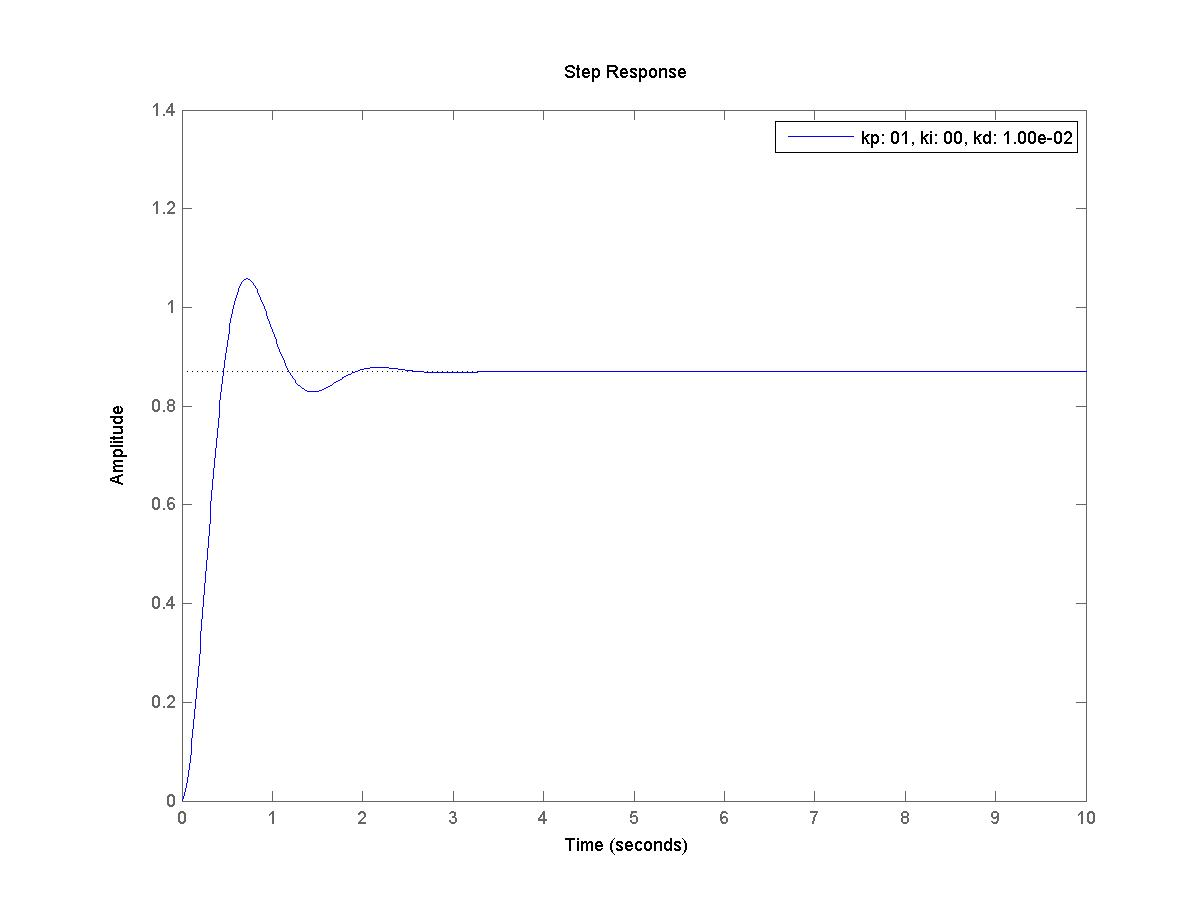
\includegraphics[width=1.8in]{part3-1.jpg} 
& 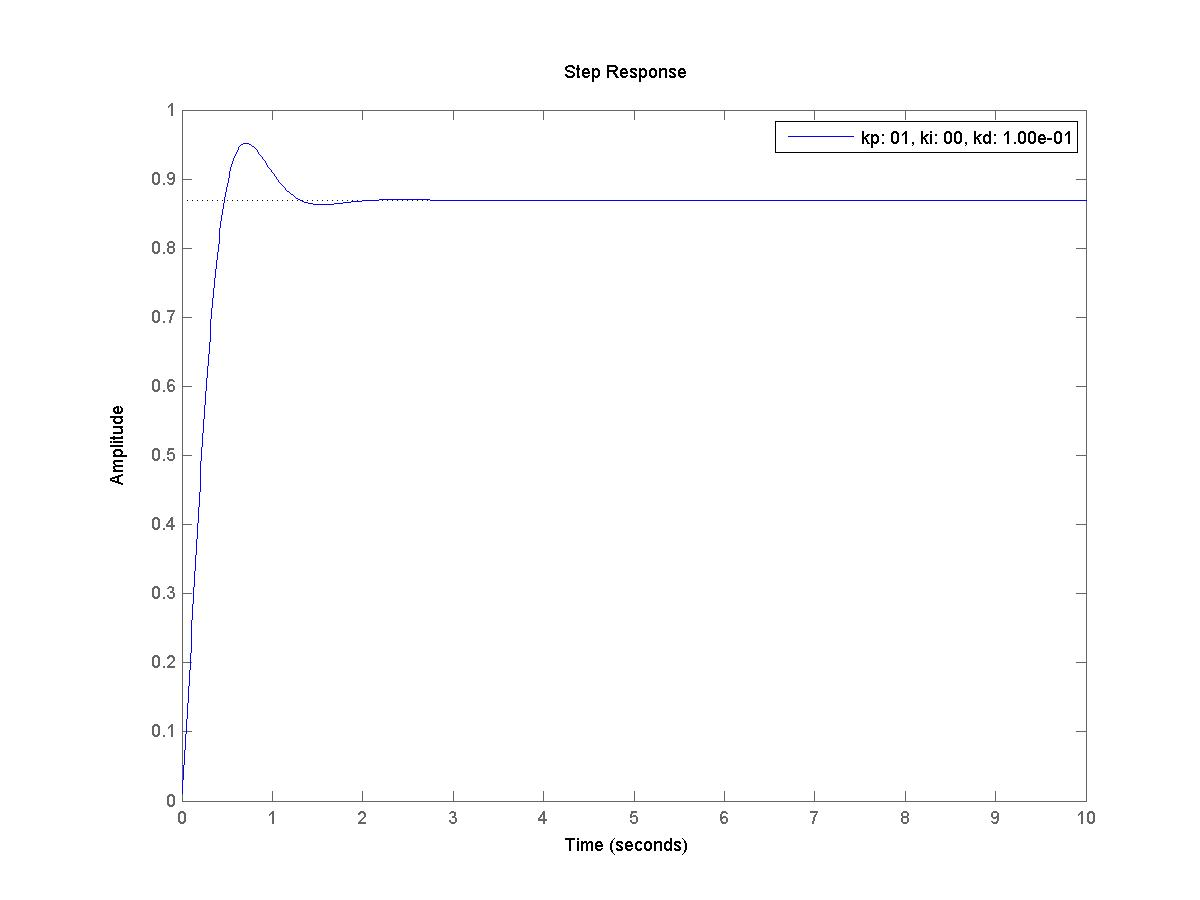
\includegraphics[width=1.8in]{part3-2.jpg} 
& 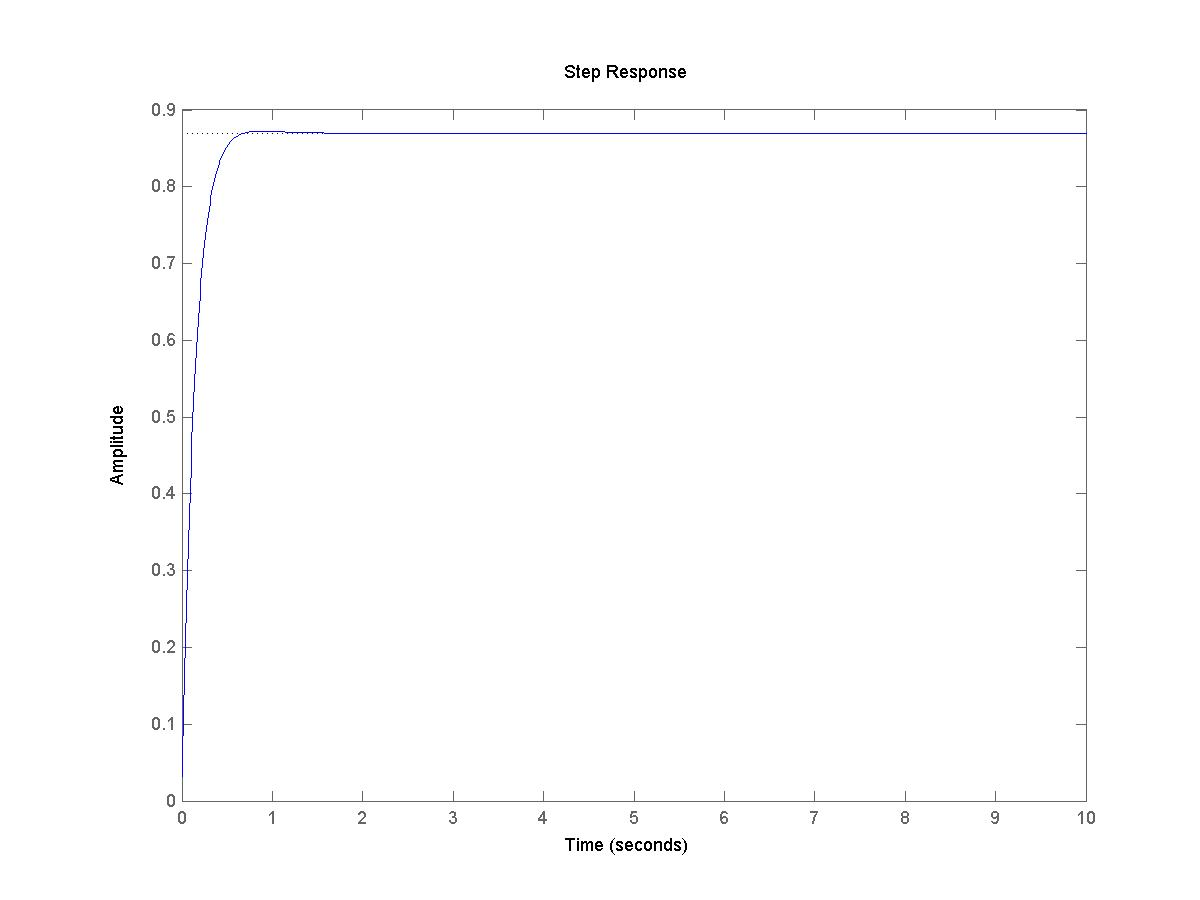
\includegraphics[width=1.8in]{part3-3.jpg} 
\\ 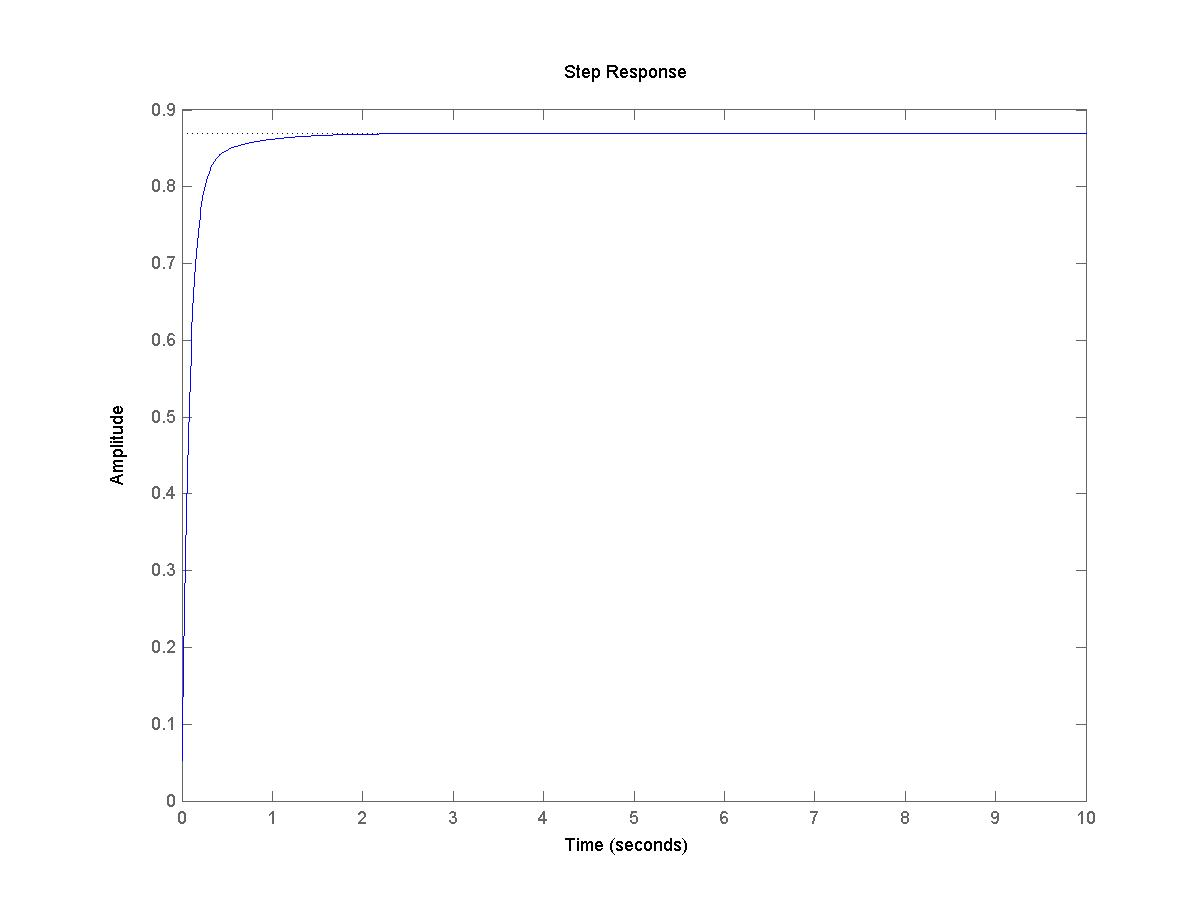
\includegraphics[width=1.8in]{part3-4.jpg} 
& 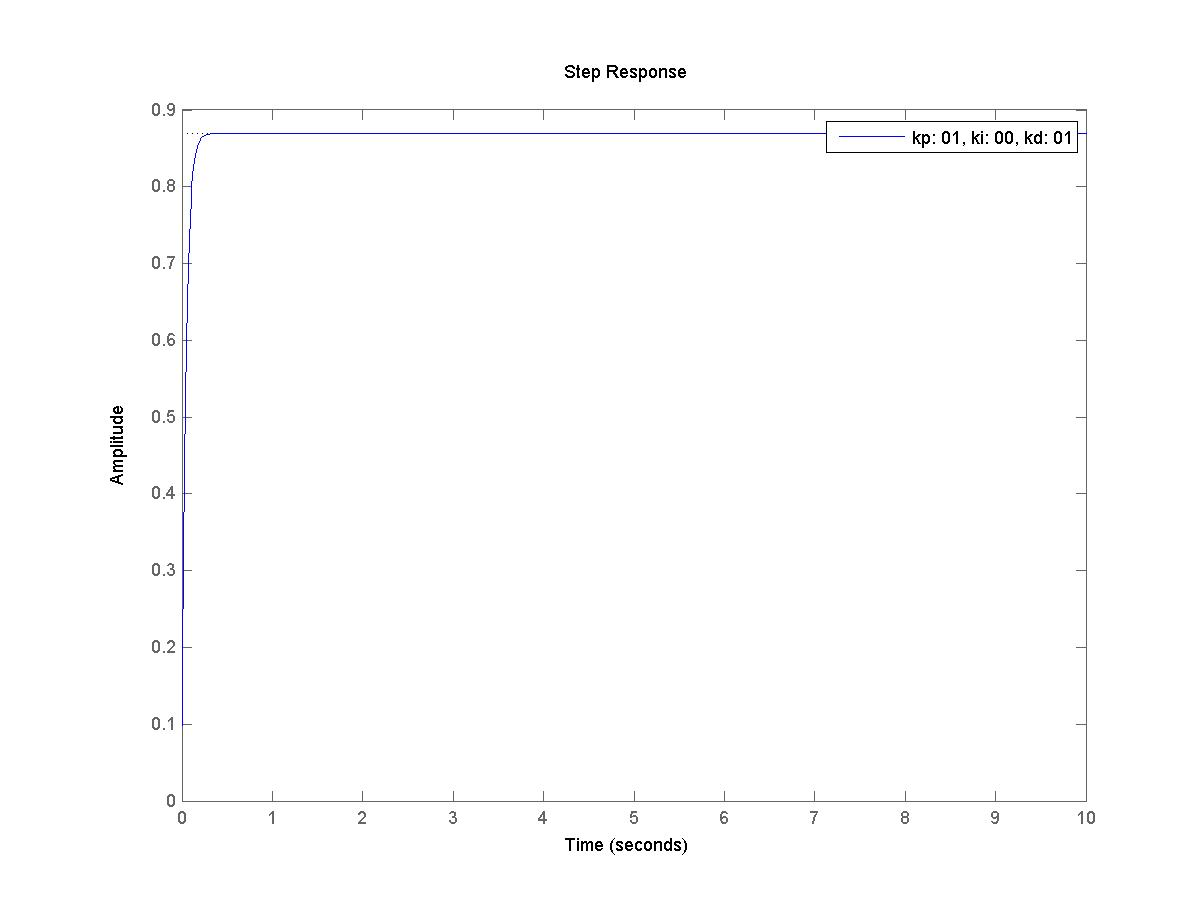
\includegraphics[width=1.8in]{part3-5.jpg} 
& 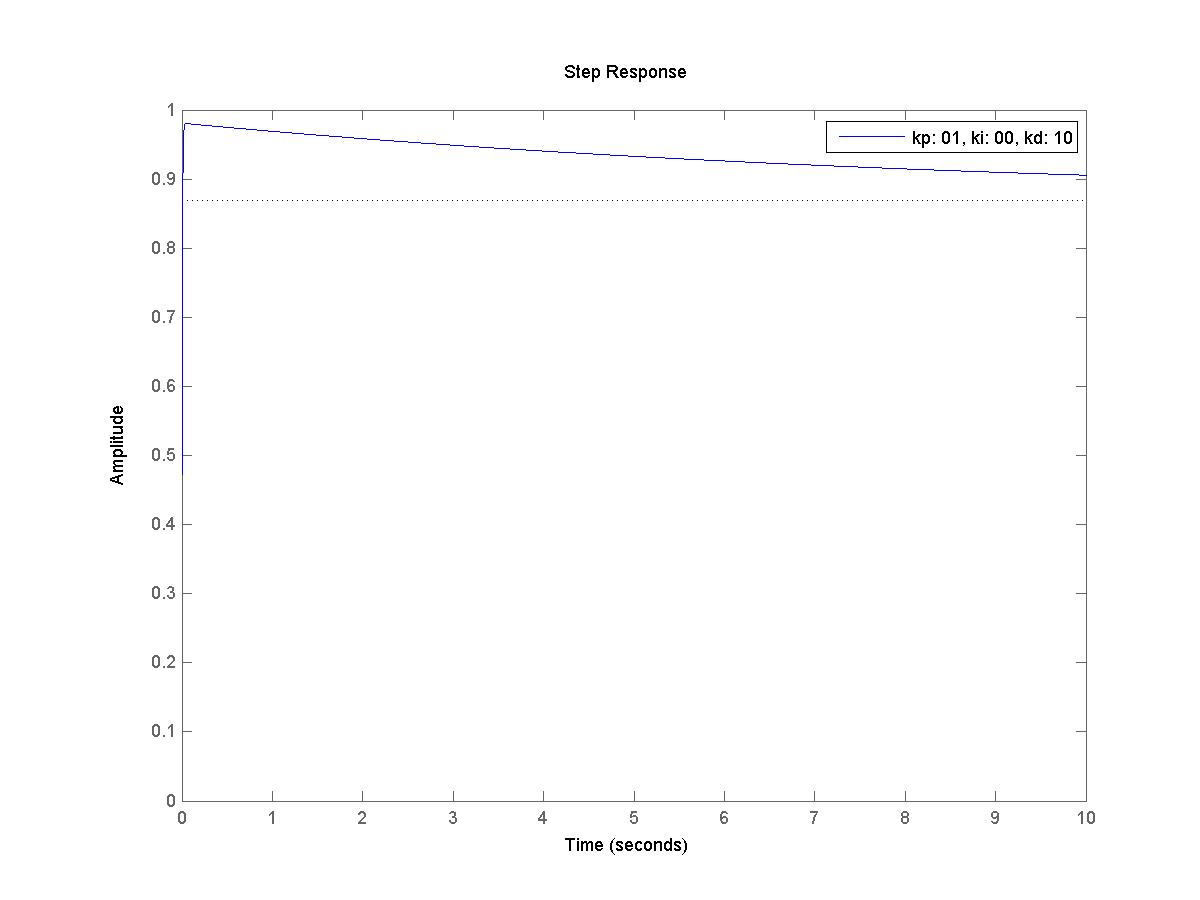
\includegraphics[width=1.8in]{part3-6.jpg} 
\\ 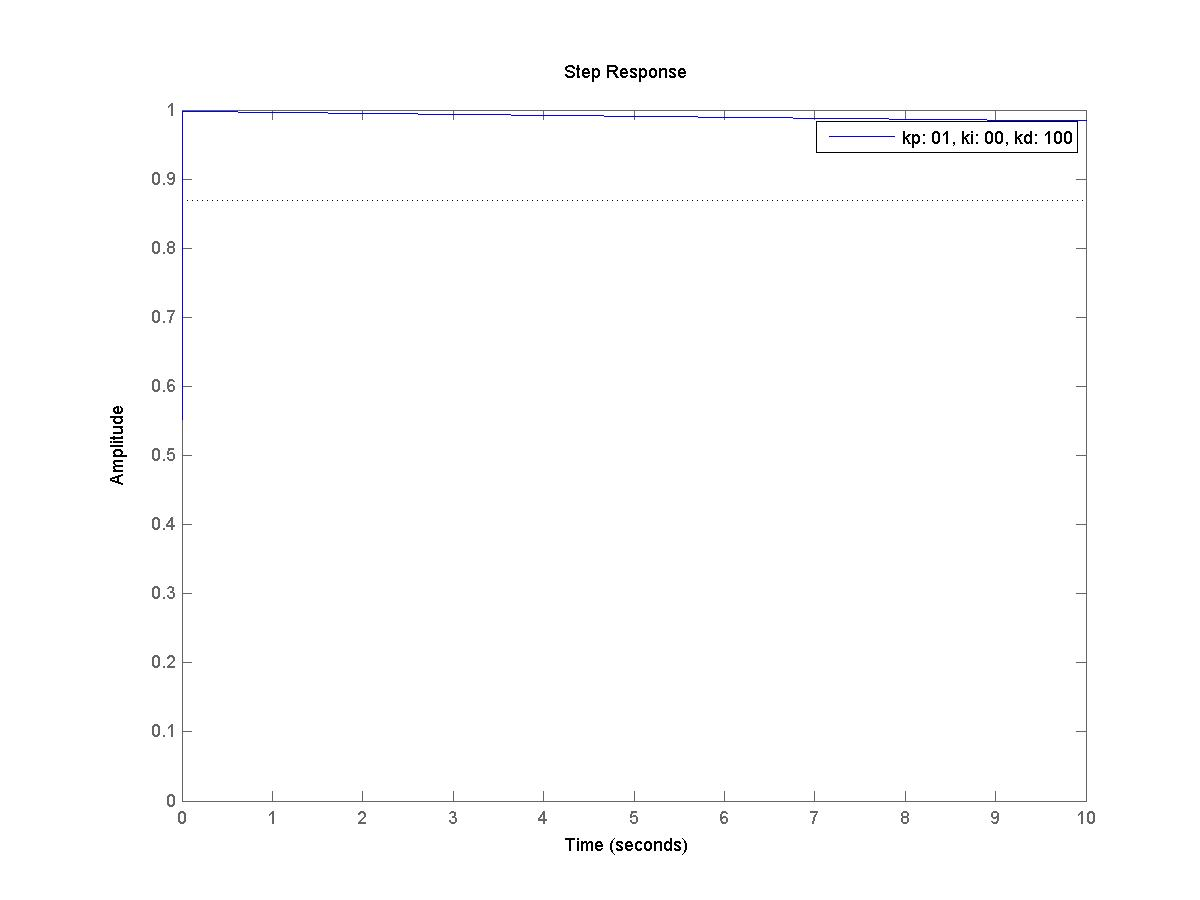
\includegraphics[width=1.8in]{part3-7.jpg} 
\\ \bottomrule
\end{tabular}
\caption{Part 3 Step Responses}
  \label{tab:part3Response}
\end{table}
\begin{table}[H]
	\begin{tabularx}{\textwidth}{XXXXXXXXXX}
		\toprule
		\\ $K_p$ & $K_i$ & $K_d$ & $T_r$ & $T_p$ & $T_s$ & $\%OS$ & $e_{ss}$ 
		& Stable System? & Damping Classification
		\\ \midrule
		
\\\midrule\\1&0&0.01&0.317&0.72&1.735&21.675&0.534&yes&under 
\\\midrule\\1&0&0.1&0.343&0.71&1.137&9.476&0.534&yes&under 
\\\midrule\\1&0&0.3&0.299&0.88&0.494&0.317&0.534&yes&critically 
\\\midrule\\1&0&0.5&0.216&0&0.587&0&0.534&yes&critically 
\\\midrule\\1&0&1&0.095&09&0.170&4.4409e-14&0.534&yes&critically 
\\\midrule\\1&0&10&0.008&0.05&6.392&8.248&0.534&yes&critically 
\\\midrule\\1&0&100&0.007&0.01&0.009&1.413&0.534&yes&critically 
		\\ \bottomrule
	\end{tabularx}
	\caption{Part 3 PID Results}
	\label{tab:pid3SimResults}
\end{table}
\begin{table}[H]
\begin{tabular}{ccc}
\toprule
\\ 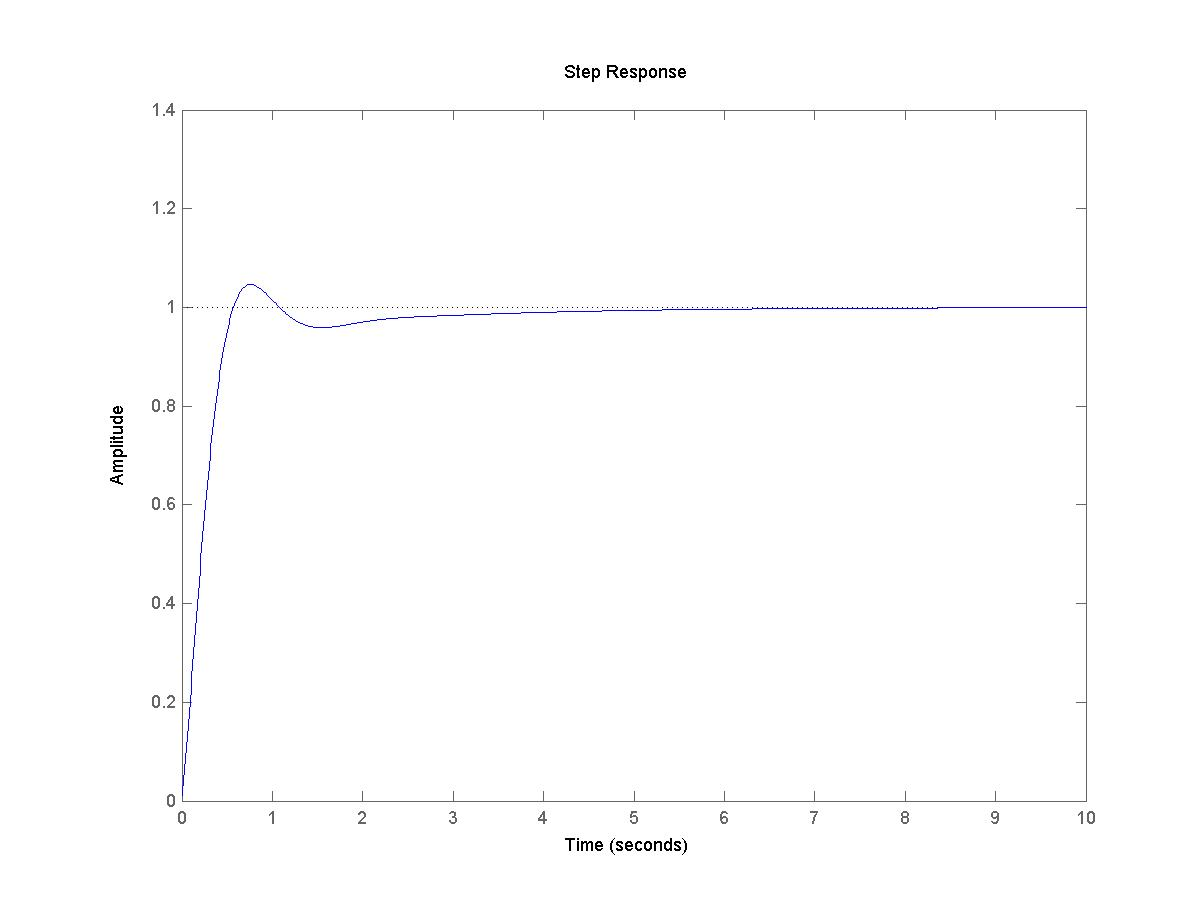
\includegraphics[width=1.8in]{part4-1.jpg} 
& 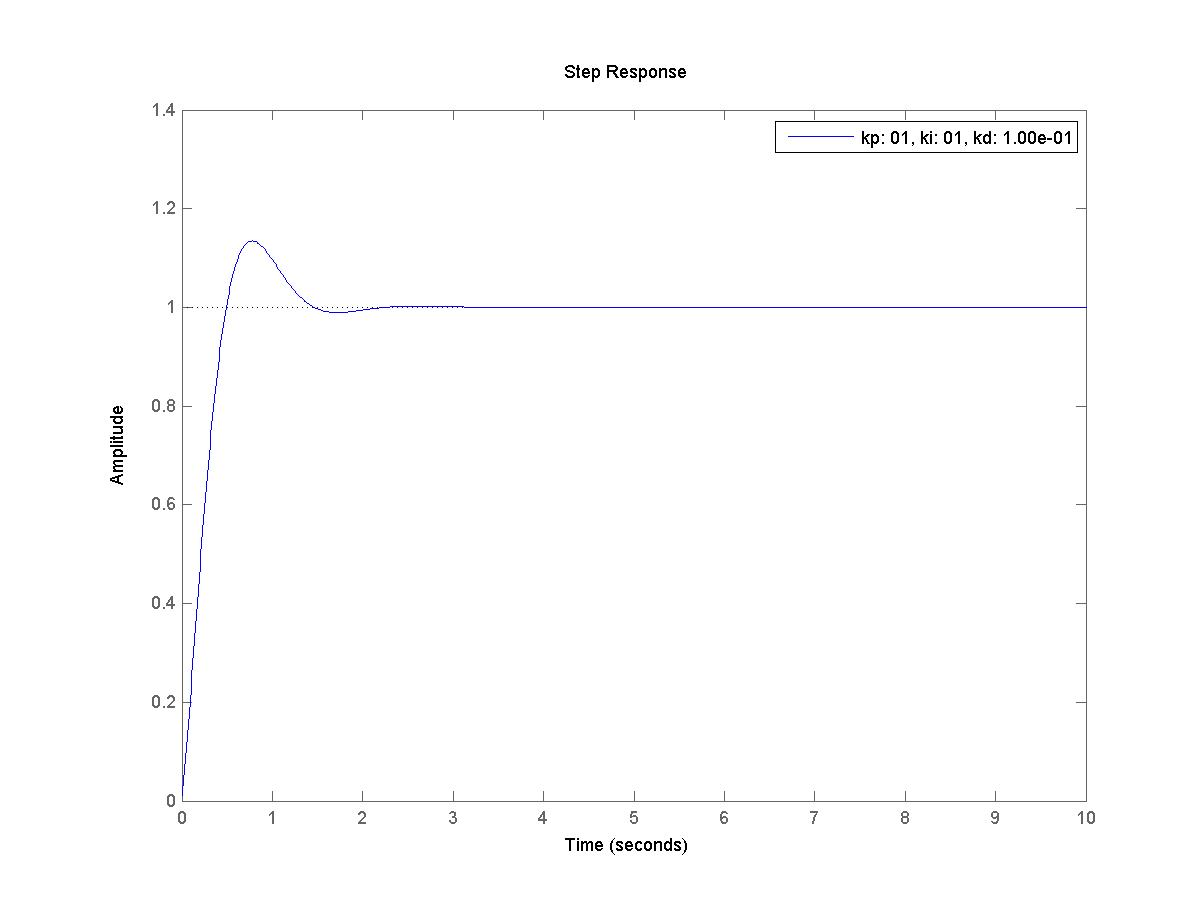
\includegraphics[width=1.8in]{part4-2.jpg} 
& 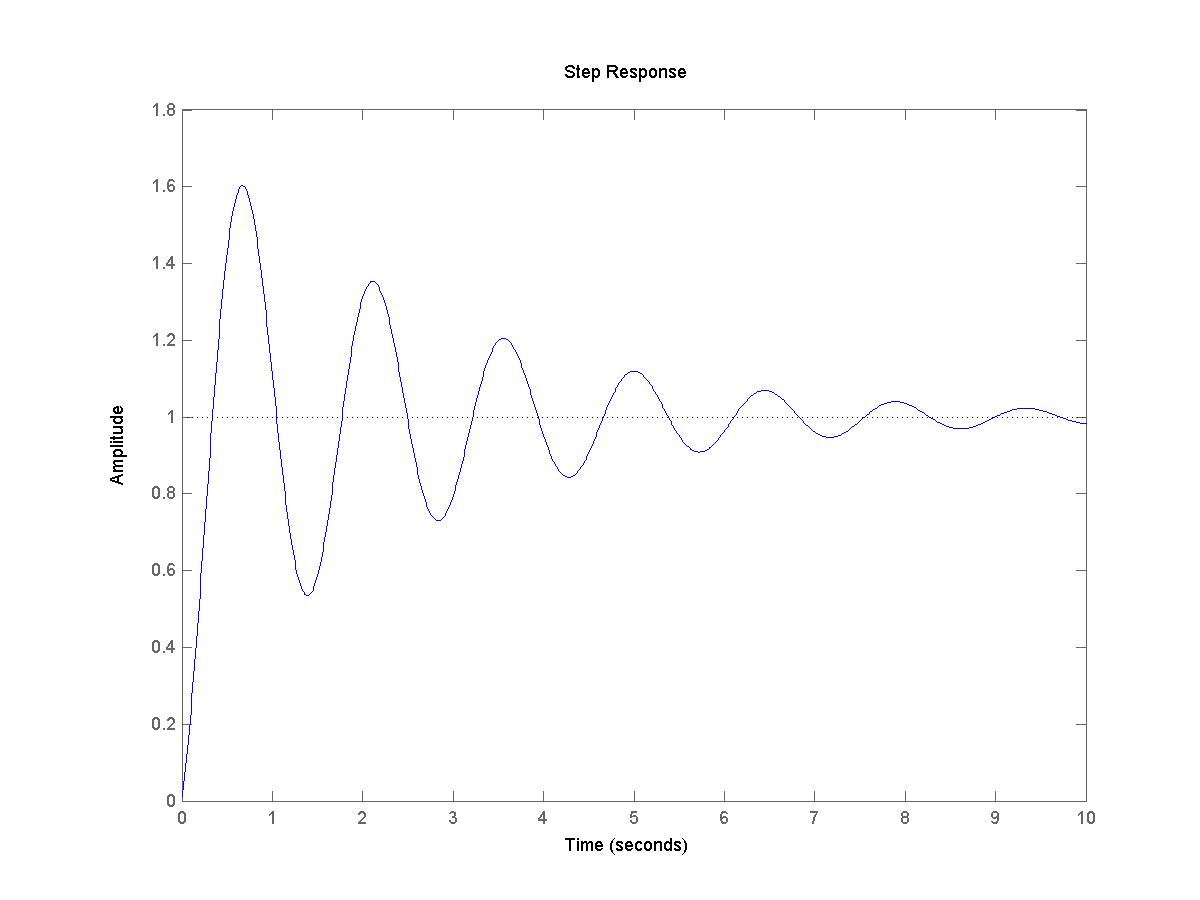
\includegraphics[width=1.8in]{part4-3.jpg} 
\\ 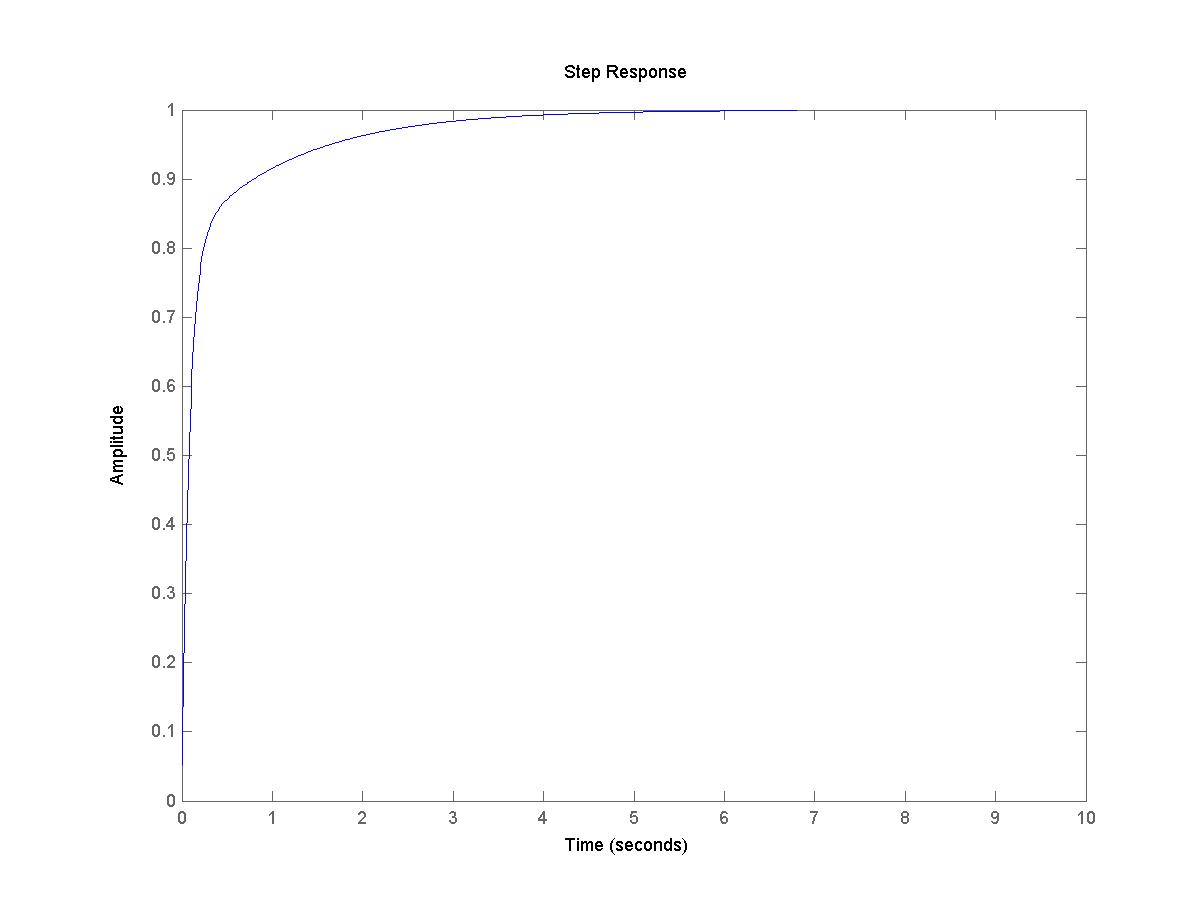
\includegraphics[width=1.8in]{part4-4.jpg} 
& 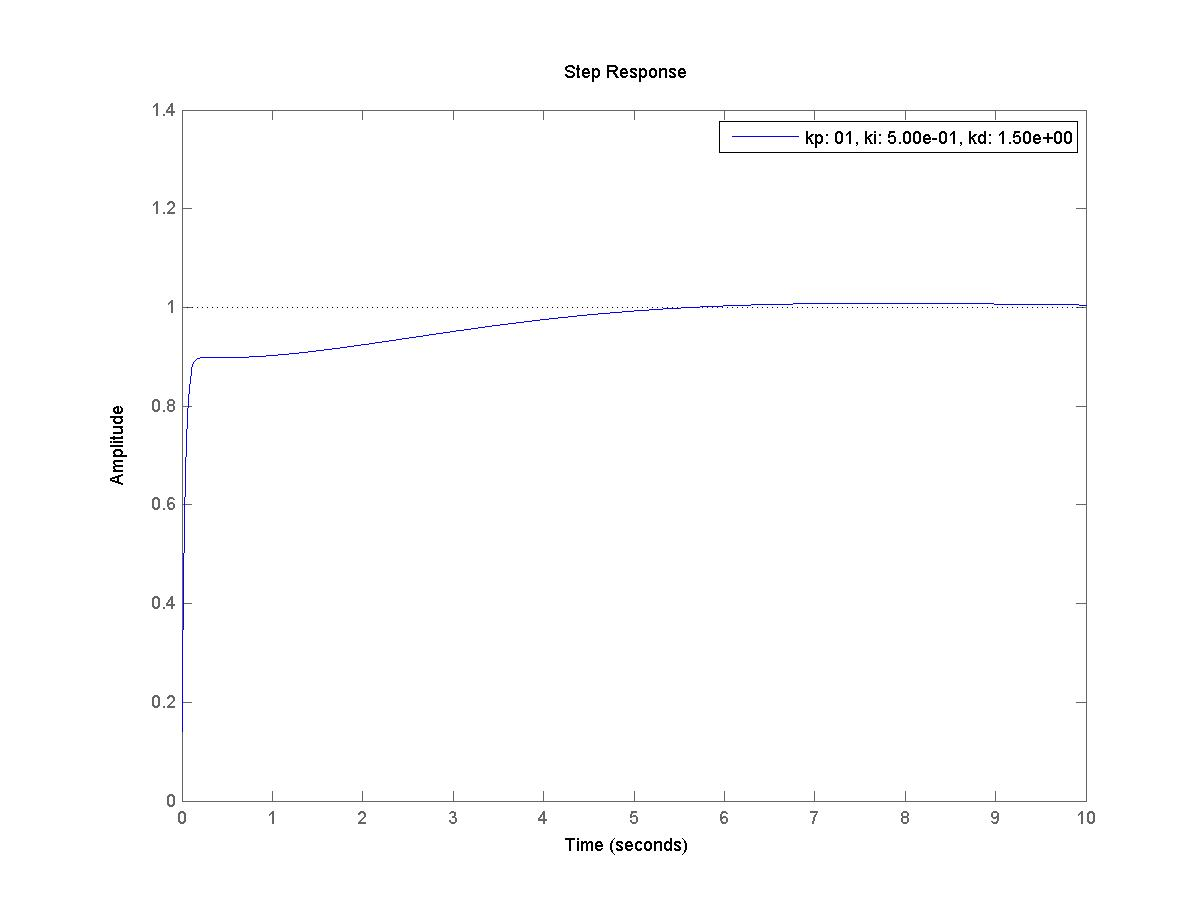
\includegraphics[width=1.8in]{part4-5.jpg} 
& 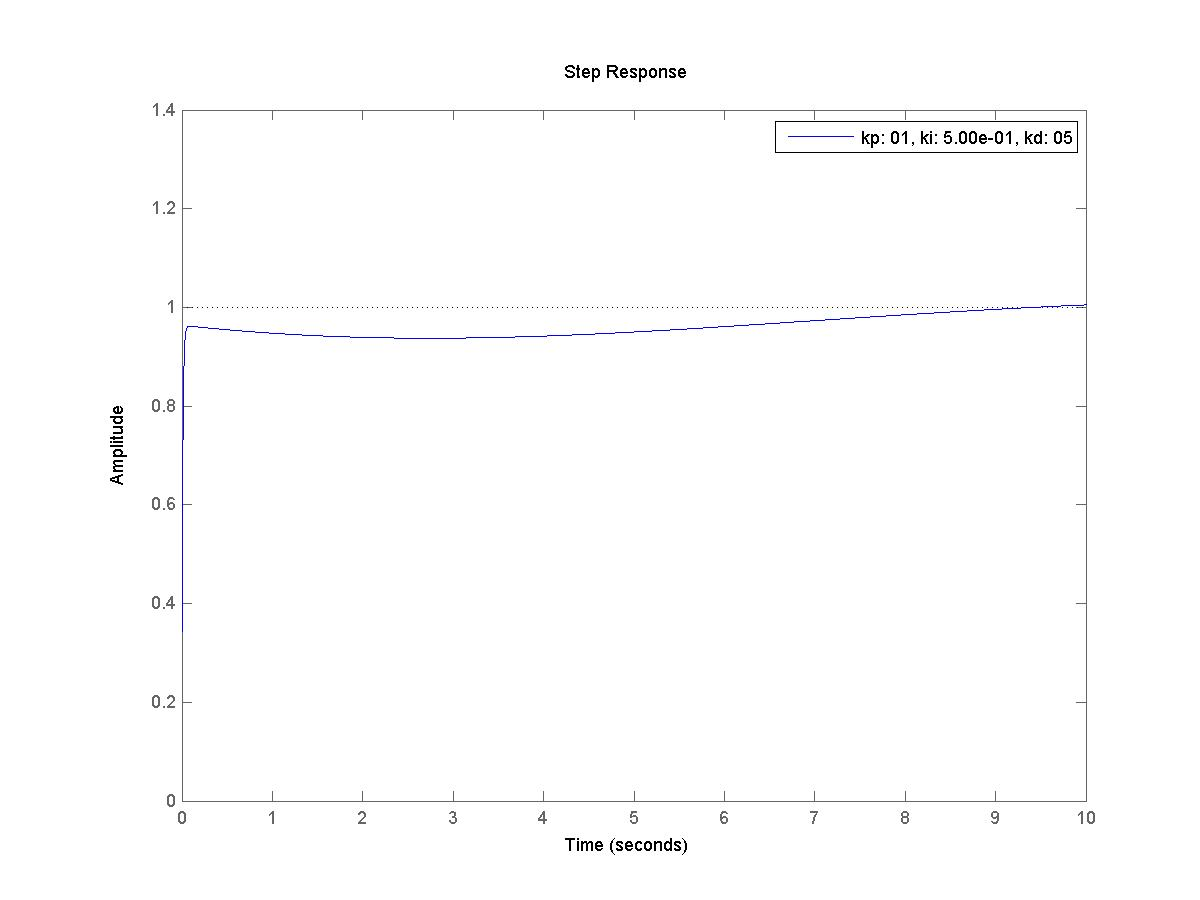
\includegraphics[width=1.8in]{part4-6.jpg} 
\\ 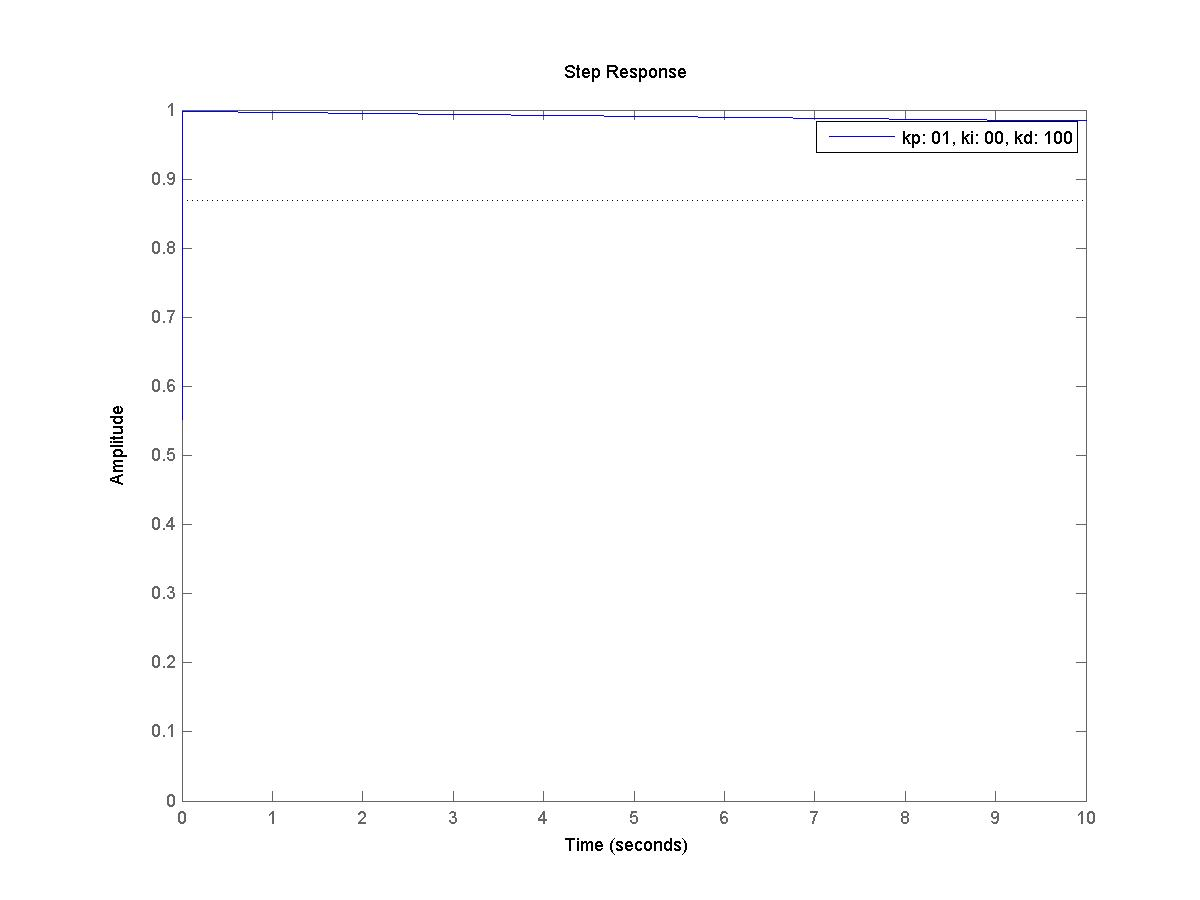
\includegraphics[width=1.8in]{part4-7.jpg} 
\\ \bottomrule
\end{tabular}
\caption{Part 4 Step Responses}
  \label{tab:part4Response}
\end{table}
\begin{table}[H]
	\begin{tabularx}{\textwidth}{XXXXXXXXXX}
		\toprule
		\\ $K_p$ & $K_i$ & $K_d$ & $T_r$ & $T_p$ & $T_s$ & $\%OS$ & $e_{ss}$ 
		& Stable System? & Damping Classification
		\\ \midrule
		
\\\midrule\\1&0.5&0.1&0.400&0.76&2.459&4.687&0.5&yes&critically 
\\\midrule\\1&1&0.1&0.365&0.78&1.315&13.46&0.5&yes&critically 
\\\midrule\\1&5&0.1&0.257&0.67&9.689&63.074&0.5&yes&under 
\\\midrule\\1&0.5&0.5&0.782&10&2.750&0&0.5&yes&critically 
\\\midrule\\1&0.5&1.5&1.099&7.73&4.487&0.366&0.5&yes&under 
\\\midrule\\1&0.5&5&0.026&10&7.988&0&0.5&yes&under 
\\\midrule\\1&0&100&0.007&0.01&0.009&1.413&0.534&yes&critically 
		\\ \bottomrule
	\end{tabularx}
	\caption{Part 4 PID Results}
	\label{tab:pid4SimResults}
\end{table}


% section results (end)

\end{document}
